\documentclass[a4paper]{article}

\usepackage[T1]{fontenc}              % Codificação para português 
\usepackage[brazilian]{babel}         % Português
\usepackage{hyphenat}                 % Use hifens corretamente
\usepackage{hyperref}                 % Links para páginas web
\usepackage{graphicx}                 % Figuras
\usepackage{float}                    % Figuras no lugar "esperado"
\graphicspath{{./images/}}            % Localização das imagens
\usepackage{fancyhdr}                 % Header estilo DCC
\setlength{\headheight}{24pt}
\usepackage{fontspec}

\title{Trabalho Prático II}
\author{Igor Lacerda Faria da Silva}
\date{\href{mailto:igorlfs@ufmg.br}{\texttt{igorlfs@ufmg.br}} }

\begin{document}

\pagestyle{fancy}
\lhead{Prof. Adriano Veloso

	Aprendizado de Máquina}
\rhead{DCC / ICEx / UFMG

	2023.1}

\maketitle

\section*{Introdução}
\label{sec:Introdução}

O objetivo deste trabalho é aprofundar o conhecimento do algoritmo de \textit{boosting}, implementando-o “do zero”. Mais especificamente, foi implementado o \textit{AdaBoost} com \textit{stumps} (árvores de decisão com apenas um nó). Como exemplo, foi analisado o \textit{dataset} \href{https://archive.ics.uci.edu/dataset/101/tic+tac+toe+endgame}{\texttt{Tic-Tac-Toe Endgame}}, que contém todos as instâncias de “Jogo da Velha” em que o jogador inicial é $x$, além do resultado do jogo. No entanto, o programa é robusto: é possível usar outros bancos de dados apenas trocando alguns parâmetros.

Foi usada validação cruzada (\textit{5-fold}) para avaliar o desempenho do modelo. Este relatório apresenta a evolução do erro variando-se a quantidade de \textit{stumps}.

\section*{Desenvolvimento}%
\label{sec:Desenvolvimento}

\begin{figure}[H]
	\begin{center}
		{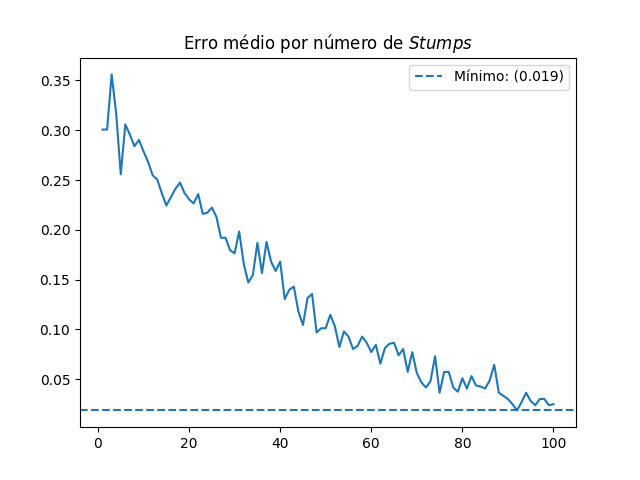
\includegraphics[height=7cm]{./images/error_per_stumps.png}}
	\end{center}
	\caption{Média do erro pelo número de \textit{stumps}, após a validação cruzada. O desempenho do modelo, de forma geral, foi satisfatório. Para até 100 stumps, o erro chegou a ser menor 2\%. \label{fig:unique}}
\end{figure}

\subsection*{Implementação}

O trabalho foi implementado em \textit{Python}. Foram usadas classes para representar os \textit{stumps} e um objeto \texttt{Dataset}, que generaliza o programa. A cada \texttt{Stump} é associado: um vetor de indices onde o \textit{stump} erra no treino (para facilitar o cálculo dos erros), um nome descritivo, uma \textit{busca} para ser realizada no \texttt{Dataset} e um alfa, para se realizar as predições. Por outro lado, o \texttt{Dataset} contém uma \textit{string} para representar o nome da coluna que contém as \textit{labels}, os possíveis valores que $x$ pode assumir, os valores ``verdadeiro'' e ``falso'' para a \textit{label} do conjunto. O próprio \textit{dataframe} é armazenado, assim como um vetor com as \textit{labels} ``ajustadas'' para -1 e 1.

O principal método do programa realiza a validação cruzada, com auxílio do \texttt{KFold} do \textit{sklearn}. Ele gera os 56 $(2*3*9+2)$\footnote{\textit{label} (verdadeiro ou falso) * possíveis valores de $x$ ('x','o','b') * número de posições + ``chutar'' tudo falso ou verdadeiro.} \textit{stumps} para cada \textit{split} com a função \texttt{gen\_stumps}, que faz as buscas nos \textit{dataframes} de treino e, principalmente, armazena os índices de erro. Em seguida, é realizado o \textit{boosting} propriamente dito, na função \texttt{boosting}. A implementação teve como inspiração os \textit{slides} da matéria e não fez nenhuma alteração relevante. Por fim, é calculado o erro, em \texttt{calculate\_test\_error}. Para fazer isso, foram usadas as \textit{queries} para se obter o valor esperado e a comparação com este poder ser realizada.

Foram realizados testes simples com base nos exemplos dos \textit{slides}, que se encontram no arquivo \texttt{src/test\_util.py}. Eles podem ser rodados com o comando \texttt{pytest}. O arquivo principal (\texttt{src/app.py}) roda a função de validação cruzada e faz um gráfico da evolução dos erros, como o adicionado neste relatório.

\end{document}
